% =====================================================================
%  ch02.tex —— 第 2 章 流形（原书 p.10–27）
%  节次：2.1 流形的定义｜2.2 用方程构造流形｜2.3 用组合构造流形
%        2.4 用商构造流形｜2.5 不可定向曲面｜2.6、2.7 附注（译文作「附注：……」）
%  陈述 46 个（含 4 个 Fact，编号 2.1–2.46 并入同一序列）；编号公式 (2.1)–(2.52)
%  图 2.1–2.3；本章无表。Fact 在 preamble 中无对应环境，按灰框 \qmstmt{事实}{n} 排版。
% =====================================================================
\setcounter{footnote}{1}

% [原文 p.10]
\chapter{流形}
\setcounter{footnote}{2}
正如已经解释的，代数拓扑给我们提供了通过给空间附加代数对象来研究空间的方法。但在做这件事之前，我们需要先了解各种值得研究的空间的例子。\footnote{优秀的数学家也许能不做任何例子，仅凭严格的数学思维过程抽象地工作。但我们不是数学家，我们确实需要例子。对数学家来说甚至有危险，如下面这则轶闻所示：https://mathoverflow.net/a/53127。长话短说，它讲的是一个数学博士论文答辩：学生证明了关于满足某些公理的对象的一大批奇妙定理。听众中的一位教授问，这样的对象是否真的存在。结果一个也没有，那些定理全部空泛地成立。}

% [原文 p.11]
为此，本节引入流形。下一节引入纤维丛，它是一类扭曲的流形乘积。代数拓扑本身从 §4 开始。

\section{流形的定义}

我们对空间有两种直觉。一种直觉是，每个点局部都像 $\R^n$。另一种是：空间由小三角形（对曲面）、小四面体（对三维对象）以及更高维的类似构造拼接而成。两种想法我们都用，但眼下主要的方法是前者。先从一些定义开始。

\begin{definition}{2.1}
一个维数为 $n$ 的（拓扑）流形 $M$ 是指这样的对象：对每个点 $p\in M$，有 $p$ 在 $M$ 中的邻域 $U\subset M$，以及 $0$ 在 $\R^n$ 中的邻域 $\ul{U}\subset\R^n$，使得存在双射连续映射 $f:U\to\ul{U}$。
\end{definition}

\begin{example}{2.2}
$\R^n$ 是 $n$ 维拓扑流形。
\end{example}

类似地，有：

\begin{definition}{2.3}
一个维数为 $n$ 的光滑流形 $M$ 是指这样的对象：对每个点 $p\in M$，有 $p$ 在 $M$ 中的邻域 $U\subset M$，以及 $0$ 在 $\R^n$ 中的邻域 $\ul{U}\subset\R^n$，使得存在双射光滑映射 $f:U\to\ul{U}$。
\end{definition}

\begin{example}{2.4}
$\R^n$ 也是 $n$ 维光滑流形。
\end{example}

在物理中，$\ul{U}$ 常称为坐标卡。我们只考虑“足够好”的流形：存在一族覆盖整个流形 $M$ 的坐标卡 $U_i$，使得对每个点 $p\in M$，只有有限个坐标卡包含 $p$。此时可以认为，流形是由坐标卡 $\ul{U}_i\subset\R^n$ 按如下方式拼接而成（见图 2.1）。假设 $U_i\cap U_j$ 非空，令
\begin{equation}
\ul{U}_{i,j} := f_i(U_i\cap U_j)\subset\ul{U}_i, \tag{2.1}
\end{equation}
\begin{equation}
\ul{U}_{j,i} := f_j(U_j\cap U_i)\subset\ul{U}_j. \tag{2.2}
\end{equation}

% [原文 p.12]
\begin{center}
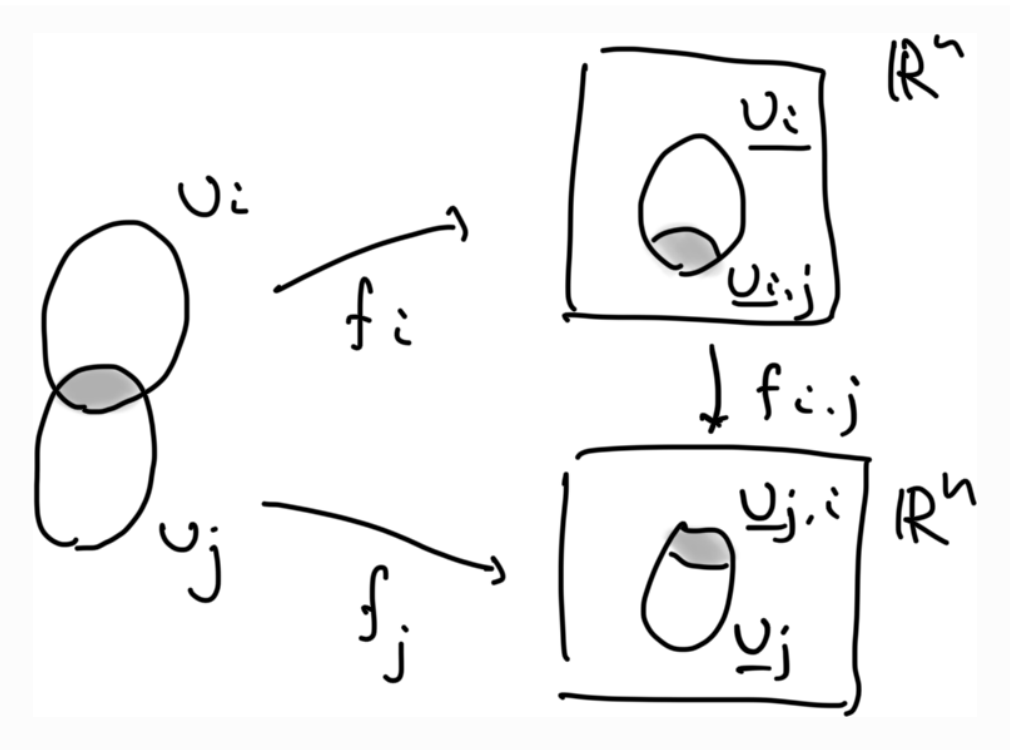
\includegraphics[width=0.62\textwidth]{figures/fig2_1.png}\\[2pt]
{\small 图 2.1：流形的坐标卡}
\end{center}

于是有映射
\begin{equation}
f_{i,j}:\ul{U}_{i,j}\to\ul{U}_{j,i}, \tag{2.3}
\end{equation}
它由下式定义：
\begin{equation}
f_{i,j} := f_j\circ(f_i)^{-1}. \tag{2.4}
\end{equation}
这让我们可以用 $f_{i,j}$ 把子集 $\ul{U}_{i,j}$ 与 $\ul{U}_{j,i}$ 等同起来，从而把 $\ul{U}_i\subset\R^n$ 与 $\ul{U}_j\subset\R^n$ “拼接”在一起。

光滑流形要求 $f_{ij}$ 光滑；拓扑流形只要求 $f_{ij}$ 连续。光滑流形自动是拓扑流形。两个光滑流形 $M$ 与 $M'$ 之间的双射光滑映射 $f:M\to M'$ 称为微分同胚；两个拓扑流形之间的双射连续映射称为同胚。物理中我们通常考虑光滑流形。但我决定也讨论一点拓扑流形，因为我想，光滑流形与拓扑流形之间那些微妙而具体的差别，可能让一些人感兴趣。

\begin{theorem}{2.5}
当流形 $M$ 紧时，可以选取有限个坐标卡 $U_i$ 覆盖 $M$。
\end{theorem}

继续之前，再引入带边流形：

\begin{definition}{2.6}
带边流形的定义类似，只是允许邻域 $\ul{U}$ 落在半空间 $\R^{n-1}\times\R_{\ge0}$ 中。把 $\ul{U}\cap(\R^{n-1}\times\{0\})$ 的边界在 $f$ 下的原像的并集称为 $M$ 的边界，记作 $\bd M$。
\end{definition}

% [原文 p.13]
例如：

\begin{example}{2.7}
半空间 $\R^{n-1}\times\R_{\ge0}$ 是带边流形。
\end{example}

\begin{definition}{2.8}
没有边界的紧流形称为闭流形。
\end{definition}

\takeaway{本节定义拓扑流形与光滑流形：每点附近同胚（或微分同胚）于 $\R^n$ 的开集，坐标卡之间由转移函数粘接。紧流形可由有限个坐标卡覆盖；允许半空间坐标卡，便得到带边流形与边界 $\bd M$。}

\section{用方程构造流形}

到此为止，我们看到的都只是平凡的例。我们需要更好的例。

\subsection{一般情形}

构造流形的一种常见方式，是取 $\R^n$ 中由若干方程定义的子集：
\begin{align}
f_1(x_1,x_2,\ldots,x_n) &= 0, \tag{2.5}\\
f_2(x_1,x_2,\ldots,x_n) &= 0, \tag{2.6}\\
&\ \vdots \tag{2.7}\\
f_m(x_1,x_2,\ldots,x_n) &= 0. \tag{2.8}
\end{align}
如果 $f_1,f_2,\ldots,f_m$ 的选取足够好，满足这些方程的点集就是 $n-m$ 维流形。

一个典型的坏例子是 $\R^2$ 中由 $xy=0$ 定义的子集：在 $(x,y)=(0,0)$ 附近两条直线相交，所以 $(0,0)$ 的邻域不是应有的形状。

\subsection{球面与圆盘}

\begin{example}{2.9}
$n$ 维球面 $S^n$ 由
\begin{equation}
x_1^2+x_2^2+\cdots+x_{n+1}^2=1 \tag{2.9}
\end{equation}
定义。注意 $S^n$ 嵌入在 $\R^{n+1}$ 中，但它本身是 $n$ 维流形。
\end{example}

\begin{example}{2.10}
$n$ 维圆盘 $D^n$ 由
\begin{equation}
x_1^2+x_2^2+\cdots+x_n^2\le 1 \tag{2.10}
\end{equation}
定义。这是带边流形，边界为 $S^{n-1}$。$D^n$ 也称为 $n$ 维球，记作 $B^n$。
\end{example}

\begin{example}{2.11}
$D^1$ 是线段 $[-1,1]$，其边界 $S^0$ 由两个点 $\{-1,1\}$ 组成。
\end{example}

把两个点 $S^0$ 称为零维球面听起来很傻，但这只是个名字。它说明了一个重要之点：不该根据名字来判断数学概念，而该把定义内化到心里来理解它们。


% [原文 p.14]
\begin{example}{2.12}
我们可以考虑 $\R^{d-1,1}$ 中到原点有固定 Lorentz 不变距离的点：
\begin{equation}
x_1^2+x_2^2+\cdots+x_{d-1}^2-x_0^2=K, \tag{2.11}
\end{equation}
其中 $K$ 是非零常数。这是双曲面，是 $d-1$ 维流形。当 $K>0$ 时它连通；这是 Minkowski 时空中到原点距离为 $\sqrt{|K|}$ 的类空间隔点构成的超曲面。当 $K<0$ 时它有两个连通分支，一个在未来 $x_0>0$，另一个在过去 $x_0<0$；它们是到原点时间距离为 $\sqrt{|K|}$ 的类时间隔点构成的超曲面。当 $K=0$ 时，上式定义光锥；光锥在原点奇异，不是流形。
\end{example}

\subsection{群流形}

我们有许多群流形，定义方式类似。

记 $M_n(\R)$ 为 $n\times n$ 实矩阵的集合。

\begin{example}{2.13}
正交群 $O(n)$ 由
\begin{equation}
O(n)=\{M\in M_n(\R)\mid M^TM=1\} \tag{2.12}
\end{equation}
定义。特殊正交群 $SO(n)$ 由
\begin{equation}
SO(n)=\{M\in O(n)\mid \det M=1\} \tag{2.13}
\end{equation}
定义。
\end{example}

类似地，记 $M_n(\C)$ 为 $n\times n$ 复矩阵的集合。

\begin{example}{2.14}
酉群 $U(n)$ 由
\begin{equation}
U(n)=\{M\in M_n(\C)\mid M^\dagger M=1\} \tag{2.14}
\end{equation}
定义。特殊酉群 $SU(n)$ 由
\begin{equation}
SU(n)=\{M\in U(n)\mid \det M=1\} \tag{2.15}
\end{equation}
定义。
\end{example}

\begin{proposition}{2.15}
$S^1=U(1)=SO(2)$。
\end{proposition}

把 $S^1$ 用 $\theta\in[0,2\pi)$ 参数化即可看出。$U(1)$ 是一阶酉矩阵，即满足 $|z|=1$ 的复数 $z$，因此 $z=e^{i\theta}$。$SO(2)$ 是行列式为 $1$ 的二阶正交矩阵，其形式为
\begin{equation}
\begin{pmatrix}\cos\theta & -\sin\theta\\ \sin\theta & \cos\theta\end{pmatrix}. \tag{2.16}
\end{equation}

% [原文 p.15]
\begin{proposition}{2.16}
$S^3=SU(2)$。
\end{proposition}

注意到任意 $SU(2)$ 矩阵都有形式
\begin{equation}
\begin{pmatrix} z & -\bar w\\ w & \bar z\end{pmatrix} \tag{2.17}
\end{equation}
且 $|z|^2+|w|^2=1$。由于 $\C^2\simeq\R^4$，可见这定义了一个 $S^3$。这个事实也可以借助四元数 $\mathbb{H}$ 来证明，四元数是 Hamilton 在 1843 年引入的。

\begin{definition}{2.17}
$\mathbb{H}$ 是 $\R$ 上的四维代数，有一组基 $1,i,j,k$，满足
\begin{equation}
\begin{gathered}
i^2=j^2=k^2=-1,\\
ij=-ji=k,\\
jk=-kj=i,\\
ki=-ik=j.
\end{gathered}\tag{2.18}
\end{equation}
\end{definition}

一般元素形如 $q=a+bi+cj+dk$，其中 $a,b,c,d\in\R$。$q=a+bi+cj+dk$ 的共轭是 $\bar q=a-bi-cj-dk$。可以验证 $\ol{q_1q_2}=\bar q_2\bar q_1$。

$q$ 的范数为 $|q|^2=q\bar q=\bar q q=a^2+b^2+c^2+d^2$。除非 $q=0$，它非零。这意味着任何非零元素 $q\neq0$ 都有乘法逆 $q^{-1}=\bar q/|q|^2$。具有此性质的代数称为可除代数。

\begin{qmbox}\qmstmt{事实}{2.18}
$\R$ 上的有限维可除代数只有 $\R$、$\C$ 和 $\mathbb{H}$。
\end{qmbox}

还要注意 $|q_1q_2|^2=|q_1|^2|q_2|^2$。这意味着单位四元数的集合 $\{q\in\mathbb{H}\mid |q|=1\}$ 构成群。由于 $\mathbb{H}\simeq\R^4$，这是三维球面 $S^3$。把 $\mathbb{H}$ 看作 $\C^2$，可以让自己相信这也是 $SU(2)$。更一般地：

\begin{example}{2.19}
酉辛群 $Sp(n)$ 由
\begin{equation}
Sp(n)=\{M\in M_n(\mathbb{H})\mid M^\dagger M=1\} \tag{2.19}
\end{equation}
定义。特别地，$Sp(1)=SU(2)=S^3$。注意并不存在另一个“特殊酉辛群”。
\end{example}

为了更几何地解释 $Sp(m)$，把 $\mathbb{H}^n$ 看作四元数列向量的空间。我们考虑“线性”映射 $M:\mathbb{H}^n\to\mathbb{H}^n$，意思是
\begin{equation}
M(vq)=(Mv)q,\qquad v\in\mathbb{H}^n,\ q\in\mathbb{H}. \tag{2.20}
\end{equation}
（注意 $q$ 放在右边很重要，因为 $\mathbb{H}$ 中乘法不交换。）把基向量记为 $e_1,e_2,\ldots,e_n$。这样的 $M$ 由
\begin{equation}
Me_i=\sum_j M_{ij}e_j \tag{2.21}
\end{equation}
确定。条件 $M^\dagger M=1$ 就是保范数的条件，其中 $v\in\mathbb{H}^n$ 的范数定义为
\begin{equation}
|v|^2:=\sum_i |v_i|^2. \tag{2.22}
\end{equation}

% [原文 p.16]
\begin{qmbox}\qmstmt{事实}{2.20}
$S^n$ 成群的情形只有 $S^0=O(1)=\{1,-1\}$、$S^1=SO(2)=U(1)$ 和 $S^3=SU(2)=Sp(1)$。
\end{qmbox}

继续之前，再引入记号：

\begin{definition}{2.21}
我们用 $GL(n,\mathbb{K})$ 表示域 $\mathbb{K}$ 上可逆 $n\times n$ 矩阵构成的群。
\end{definition}

\subsection{附注：时间反演与 $\R$、$\C$、$\mathbb{H}$}

让我就 $\mathbb{H}$ 在量子力学中的自然作用做一点旁注。考虑一个具有有限维 希尔伯特空间 $\mathcal{H}$ 的量子力学系统。时间反演算子 $\mathrm{T}$ 是反酉的，即
\begin{equation}
\mathrm{T} z=\bar z\,\mathrm{T}. \tag{2.23}
\end{equation}
假设 $\mathrm{T}^2=c$，其中 $c$ 是常数，我们来证明 $c=\pm1$。用两种顺序计算 $\mathrm{T}^3$：
\begin{equation}
\mathrm{T}(\mathrm{T}^2)=\mathrm{T}c=c\,\mathrm{T},\qquad (\mathrm{T}^2)\mathrm{T}=c\,\mathrm{T}. \tag{2.24}
\end{equation}
因此 $c=\bar c$。而 $\mathrm{T}^2$ 的酉性要求 $|c|=1$，所以 $c=\pm1$。

\para{情形 $c=+1$：}此时任何向量 $v\in\mathcal{H}$ 都可以分解为实部与虚部：
\begin{equation}
v=v_{\mathrm{re}}+v_{\mathrm{im}}i \tag{2.25}
\end{equation}
其中
\begin{equation}
v_{\mathrm{re}}:=\frac{1+\mathrm{T}}{2}v,\qquad v_{\mathrm{im}}:=\frac{1-\mathrm{T}}{2i}v. \tag{2.26}
\end{equation}
注意 $\mathrm{T}v_{\mathrm{re}}=v_{\mathrm{re}}$、$\mathrm{T}v_{\mathrm{im}}=v_{\mathrm{im}}$。所以 $\mathcal{H}$ 中 $\mathrm{T}$-不变的部分是实向量空间。记它为 $\mathcal{H}_\R$，则若 $\mathcal{H}_\R=\R^n$，就有 $\mathcal{H}=\C^n$。作用在 $\mathcal{H}$ 上且与 $\mathrm{T}$ 交换的酉矩阵，就是作用在 $\mathcal{H}_\R$ 上的正交矩阵。因此，$\mathcal{H}$ 上时间反演不变的酉算子构成群 $O(n)$。

\para{情形 $c=-1$：}此时注意 $i$、$j:=\mathrm{T}$、$k:=i\mathrm{T}$ 满足 $\mathbb{H}$ 的定义关系 (2.18)。（更确切地说，我们可以通过 $vi:=iv$、$vj:=\mathrm{T}v$ 从右边赋予量子态空间 $\mathcal{H}$ 一个 $\mathbb{H}$ 的作用。）因此 $\mathcal{H}=\mathbb{H}^m$ 对某个 $m$ 成立。当 $\mathcal{H}=\C^n$ 时，这迫使 $n=2m$ 为偶数。这称为 Kramers 简并。

与 $\mathrm{T}$ 交换的酉算子是 $\mathbb{H}^m$ 上的保范映射，且与从右边的四元数作用交换。因此它属于 $Sp(m)$。

% [原文 p.17]
\para{总结：}$U(n)$、$SO(n)$ 与 $Sp(n/2)$ 是 $n$ 个态的量子系统 $\mathcal{H}=\C^n$ 上保范线性算子构成的群，分别对应以下条件：
\begin{itemize}
\item $U(n)$：没有时间反演；
\item $SO(n)$：有时间反演，且 $\mathrm{T}^2=+1$；
\item $Sp(n/2)$：有时间反演，且 $\mathrm{T}^2=-1$；此时 $n$ 被迫为偶数。
\end{itemize}

\takeaway{本节用方程构造流形：$\R^n$ 中 $m$ 个合适方程的公共零点集是 $n-m$ 维流形，由此得到球面、圆盘、Lorentz 双曲面与群流形 $O(n)$、$U(n)$、$Sp(n)$。四元数解释 $S^3=SU(2)$，时间反演说明 $O(n)$、$U(n)$、$Sp(n/2)$ 的来历。}

\section{用组合构造流形}

回到流形的例子。

\begin{notation}{2.22}
给定两个流形 $M$、$N$，维数分别为 $m$、$n$，记它们的乘积为 $M\times N$。它是 $m+n$ 维流形。
\end{notation}

\begin{notation}{2.23}
给定两个维数同为 $n$ 的流形 $M$、$N$，记它们的不交并为 $M\sqcup N$。它是 $n$ 维流形。
\end{notation}

注意 $S^1\times S^1$ 是二维的，是甜甜圈的表面；而 $S^1\sqcup S^1$ 由两个圆组成，是一维的。

\begin{example}{2.24}
$n$ 维环面为
\begin{equation}
T^n=\overbrace{S^1\times S^1\times\cdots\times S^1}^{n\ \text{个}}. \tag{2.27}
\end{equation}
\end{example}

\begin{example}{2.25}
$S^1\times[-1,1]$ 是圆柱面。它的边界是 $S^1\sqcup S^1$。
\end{example}

另一种构造如下：

\begin{notation}{2.26}
给定两个 $n$ 维连通流形 $M$、$N$，取点 $p\in M$、$q\in N$。从 $M$ 与 $N$ 中分别挖去小开球 $B^n(p)$ 与 $B^n(q)$，再把公共边界 $S^{n-1}$ 粘起来。结果就是连通和 $M\#N$。
\end{notation}

例如，连通和
\begin{equation}
\overbrace{T^2\#T^2\#\cdots\#T^2}^{g\ \text{个}} \tag{2.28}
\end{equation}
是多甜甜圈（multi-donut）的表面（不管那是什么东西）。更专业地说，它称为亏格 $g$ 曲面。$S^2$ 的亏格定为 0。

% [原文 p.18]
\begin{qmbox}\qmstmt{事实}{2.27}
任何二维紧连通可定向流形要么是 $S^2$，要么是带 $g$ 个洞的多甜甜圈表面。
\end{qmbox}

\takeaway{本节用组合操作造流形：乘积、不交并与连通和。$T^n$ 是 $n$ 个圆的乘积；亏格 $g$ 曲面是 $g$ 个环面的连通和。二维紧连通可定向流形只有球面与亏格 $g$ 曲面。}

\section{用商构造流形}

\subsection{一般情形}

定义流形的另一种方法，是取流形对群作用的商。我们更完整地解释一下。

\begin{definition}{2.28}
群 $G$ 在流形 $M$ 上的群作用是一个映射
\begin{equation}
M\times G\to M,\qquad (p,g)\mapsto pq \tag{2.29}
\end{equation}
使得
\begin{equation}
pe=p,\qquad (pg)h=p(gh) \tag{2.30}
\end{equation}
对所有 $g,h\in G$、$p\in M$ 成立。这里 $e$ 是 $G$ 的单位元。这种情形常简记为 $M\curvearrowleft G$。
\end{definition}

更确切地说，这称为 $G$ 的右作用。类似地可以定义 $G$ 的左作用，即有映射 $G\times M\to M$ 满足 $g(hp)=(gh)p$。此时记作 $G\curvearrowleft M$。无论哪种情形，我们通常都希望作用是光滑的，或至少连续的，视语境而定。

向量空间上的群表示是特殊情形：

\begin{definition}{2.29}
群 $G$ 在 $\mathbb{K}$-向量空间 $V$ 上的表示 $\rho$，是 $G$ 在 $V$ 上的（左）群作用，且与 $\mathbb{K}$ 的标量乘法（从右边）交换。这意味着对每个 $g\in G$，有线性映射 $\rho(g):V\to V$，使得 $\rho(gh)=\rho(g)\rho(h)$。这种情形常简记为 $\rho:G\curvearrowright V$。
\end{definition}

现在定义商：

\begin{definition}{2.30}
对 $p,q\in M$，若存在 $g\in G$ 使 $pg=q$，就记 $p\sim q$。商空间 $M/G$ 是此等价关系下的等价类集合 $M/{\sim}$。
\end{definition}

$M/G$ 不总是流形。例如，考虑 $\R^3$ 上由
\begin{equation}
(x,y,z)\mapsto(-x,-y,-z) \tag{2.31}
\end{equation}
生成的 $\Z_2$ 作用。原点是奇异的，商空间 $\R^3/\Z_2$ 不是流形，但仍属于一类更大的空间，称为轨形（orbifold）。事实上，向量空间对经由其表示给出的群作用的商，几乎从来不是流形。$M/G$ 成为流形的条件陈述起来很复杂，本系列讲义中不讨论。

% [原文 p.19]
\subsection{射影空间}

现在统一地定义实、复、四元数射影空间 $\RP^n$、$\CP^n$ 与 $\HP^n$。

\begin{example}{2.31}
对 $\mathbb{K}=\R,\C,\mathbb{H}$，考虑 $\mathbb{K}\setminus\{0\}$ 通过标量乘法作用在 $\mathbb{K}^{n+1}\setminus\{0\}$ 上（当 $\mathbb{K}=\mathbb{H}$ 时从右边作用）。射影空间 $\mathbb{K}P^n$ 定义为
\begin{equation}
\mathbb{K}P^n=(\mathbb{K}^{n+1}\setminus\{0\})/(\mathbb{K}\setminus\{0\}). \tag{2.32}
\end{equation}
它们的维数分别为 $n$、$2n$ 和 $4n$。
\end{example}

更直接地，我们考虑元素
\begin{equation}
(x_1,x_2,\ldots,x_{n+1})\in\mathbb{K}^{n+1}, \tag{2.33}
\end{equation}
其中并非所有 $x_i$ 都为零。然后作等同
\begin{equation}
(x_1,x_2,\ldots,x_{n+1})\sim(x_1,x_2,\ldots,x_{n+1})c \tag{2.34}
\end{equation}
其中 $c\in\mathbb{K}$ 非零。% [Tutor Note: 原文式 (2.34) 右端误印作 (x_0,x_1,\ldots,x_n)c，按上下文应为 (x_1,\ldots,x_{n+1})c，译文从后者。]
$\mathbb{K}P^n$ 上的点（即 (2.34) 下的等价类）常记为
\begin{equation}
[x_1:x_2:\cdots:x_{n+1}]. \tag{2.35}
\end{equation}

给出显式的坐标卡是有启发性的。令 $U_i$ 为 $\mathbb{K}P^n$ 中满足 $x_i\neq0$ 的点。注意当 $x_i\neq0$ 时，有
\begin{equation}
(x_1,x_2,\ldots,x_{n+1})\sim(x_1/x_i,x_2/x_i,\ldots,x_i/x_i=1,\ldots,x_{n+1}/x_i). \tag{2.36}
\end{equation}
换言之，我们可以通过定义 $y_k:=x_k/x_i$（$k\neq i$）在 $U_i$ 上引入坐标；等价地说，我们构造了映射 $f_i:U_i\to\ul{U}_i\simeq\mathbb{K}^n$。

考虑另一个坐标卡 $U_j$，它包含满足 $x_j\neq0$ 的点。引入坐标 $z_k:=x_k/x_j$（$k\neq j$），这给出映射 $f_j:U_j\to\ul{U}_j\simeq\mathbb{K}^n$。

$U_i$ 与 $U_j$ 在 $x_i\neq0$ 且 $x_j\neq0$ 时重叠。此时需要找出 $f_i(U_i\cap U_j)\subset\ul{U}_i$ 与 $f_j(U_i\cap U_j)\subset\ul{U}_j$ 之间的坐标变换，实现
\begin{equation}
(y_1,y_2,\ldots,y_{n+1})\quad\text{其中 } y_i=1,\ y_j\neq0 \tag{2.37}
\end{equation}
与
\begin{equation}
(z_1,z_2,\ldots,z_{n+1})\quad\text{其中 } z_j=1,\ z_i\neq0 \tag{2.38}
\end{equation}
的等同。这通过令 $z_k=y_k/y_j$ 实现，其中 $y_i$ 已被定义为 $1$。

从这一描述可以看出
\begin{equation}
\RP^1=S^1,\qquad \CP^1=S^2,\qquad \HP^1=S^4. \tag{2.39}
\end{equation}
确实，此时我们有两个坐标卡
\begin{equation}
U_1=\{[1:y]\mid y\in\mathbb{K}\},\qquad U_2=\{[z:1]\mid z\in\mathbb{K}\}. \tag{2.40}
\end{equation}

% [原文 p.20]
其中 $z=y^{-1}$ 定义在重叠 $U_1\cap U_2$ 上。$U_1$ 是北半球，$U_2$ 是南半球，它们粘起来构成相应维数的球面。

看 $\mathbb{K}P^n$ 的另一种方式如下。为了在等同 (2.34) 下选取代表元，我们先固定 $\sum_i|x_i|^2=1$。由于 $\mathbb{K}^{n+1}=\R^{p(n+1)}$，其中 $p=1,2,4$ 分别对应 $\mathbb{K}=\R,\C,\mathbb{H}$，此时得到 $S^n$、$S^{2n+1}$、$S^{4n+3}$。

等同 (2.34) 在 $|c|=1$ 时仍作用在这个球面内。取决于 $\mathbb{K}=\R,\C,\mathbb{H}$，这样的 $c$ 构成的群分别是 $O(1)=\{\pm1\}=S^0$、$U(1)=S^1$、$Sp(1)=SU(2)=S^3$。因此有

\begin{proposition}{2.32}
$\RP^n=S^n/O(1)$，$\CP^n=S^{2n+1}/U(1)$，$\HP^n=S^{4n+3}/Sp(1)$。
\end{proposition}

\begin{remark}{2.33}
在继续之前，注意 $\CP^n$ 参数化了 $(n+1)$ 维 希尔伯特空间中物理上不同的纯态。确实，两个非零 ket 向量 $|\psi\rangle$ 与 $|\psi'\rangle$ 表示同一物理态，当且仅当存在复数 $c$ 使 $|\psi'\rangle=c|\psi\rangle$。这正好是条件 (2.34)。
\end{remark}

\subsection{齐性空间}

\para{一般情形：}又一大类商空间是齐性空间。

\begin{definition}{2.34}
给定子群 $H\subset G$，引入等价关系：若存在 $h\in H$ 使 $g_1=g_2h$，则 $g_1\sim g_2$。$G$ 对此关系的商记作 $G/H$，称为齐性空间。
\end{definition}

齐性空间在物理中出现的一种常见方式是通过对称性破缺。设有位形空间 $M$（通常是向量空间），对称群 $G$ 从左作用：$M\ni m\mapsto gm\in M$，$g\in G$。设有一个在 $G$ 作用下不变的势（或自由能）$V:M\to\R$，即 $V(gm)=V(m)$。再设势在 $m_0\in M$ 处取极小。由 $G$-不变性，形如 $gm_0$ 的所有点也是 $V$ 的极小点。当势是一般的时候，势的极小点空间由轨道 $Gm_0$ 给出。关于这个空间的结构，我们能多说些什么？

设 $H\subset G$ 是固定 $m_0$ 的子群，即 $h\in H$ 当且仅当 $hm_0=m_0$。这种情形下，我们说对称性从 $G$ 破缺到 $H$。\footnote{物理学家常把它写成 $G\to H$，但数学上映射的方向相反，是 $H\to G$。}此时 $g_1m_0=g_2m_0$ 当且仅当 $g_2^{-1}g_1\in H$；等价地，存在 $h\in H$ 使 $g_1=g_2h$。因此 $Gm_0=G/H$。也就是说，势的极小点空间是由原对称性 $G$ 与未破缺对称性 $H$ 决定的齐性空间。

注意数学家把子群 $H$ 称为 $m_0$ 的稳定化子，而物理学家通常称它为未破缺子群。

\para{酒瓶势：}先给一些例子。我们从两个平凡的例开始。令 $G=SO(2)$ 通过旋转作用在 $(x,y)\in\R^2$ 上。旋转不变的势 $V(x,y)$ 具有形式 $V(x,y)=f(r)$，其中 $r^2=x^2+y^2$。当极小值在 $(x,y)=(0,0)$ 处时，它在 $SO(2)$ 下的轨道是单点 $\{(0,0)\}$。此时未破缺子群 $H$ 是整个 $SO(2)$。于是 $SO(2)/SO(2)=\{\text{点}\}$，即由单点构成的零维流形。代数拓扑中常简记为 $\pt$，所以 $SO(2)/SO(2)=\pt$。

当极小值在 $(x,y)=(r_0,0)$ 处且 $r_0\neq0$ 时，它在 $SO(2)$ 下的轨道是半径为 $r_0$ 的圆。此时未破缺子群 $H$ 是 $\{e\}$，而 $SO(2)/\{e\}=SO(2)$ 是一个圆。图示见图 2.2。

% [原文 p.21]
\begin{center}
\begin{minipage}{\textwidth}
\centering
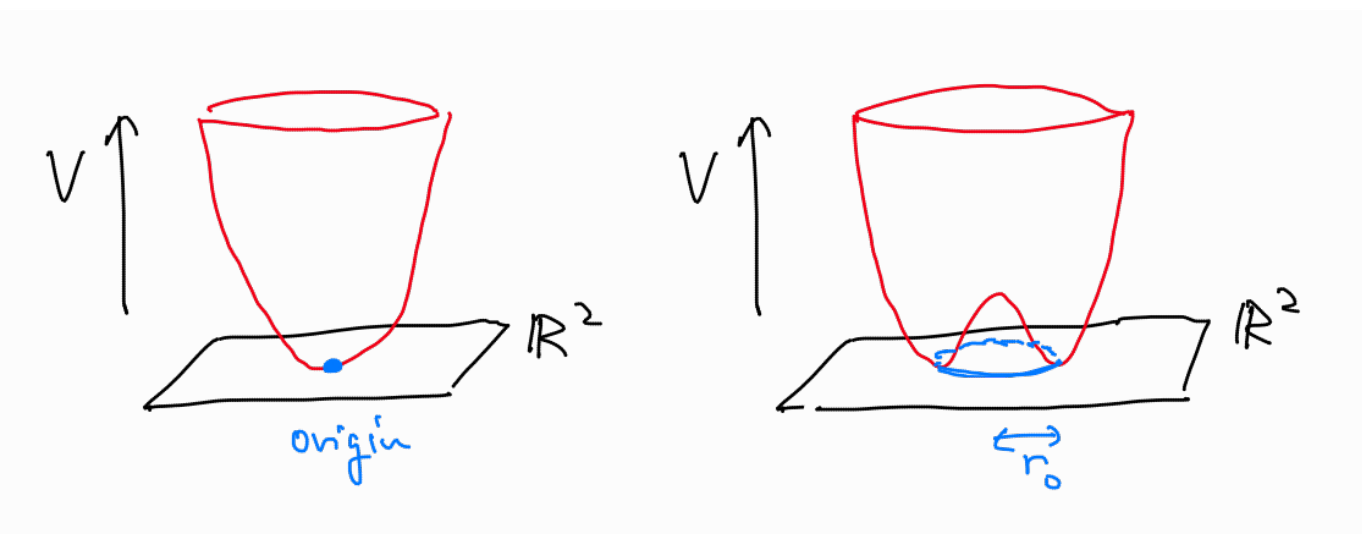
\includegraphics[width=0.62\textwidth]{figures/fig2_2.png}\\[2pt]
{\small 图 2.2：$SO(2)$-不变势 $V$ 的两例，极小值在原点与半径 $r_0$ 的圆上}
\end{minipage}
\end{center}

\para{广义酒瓶：}我们来推广。令 $SO(n)$ 通过旋转作用在 $\R^n$ 上。旋转不变的势 $V:\R^n\to\R$ 具有形式 $V(x_1,\ldots,x_n)=f(r)$，其中 $r^2=x_1^2+\cdots+x_n^2$。当 $f(r)$ 在 $r_0>0$ 处取极小值时，势取极小的空间是由 $x_1^2+\cdots+x_n^2=r_0^2$ 给出的 $S^{n-1}$。

在 $m_0=(r_0,0,\ldots,0)$ 处，固定 $m_0$ 的 $SO(n)$ 的子群是 $SO(n-1)$。因此势取极小的空间是 $SO(n)/SO(n-1)=S^{n-1}$。总结起来，我们得到

\begin{proposition}{2.35}
$SO(n)/SO(n-1)\simeq S^{n-1}$。
\end{proposition}

令 $U(n)$ 通过酉变换作用在 $\C^n$ 上。不变的势 $\C^n\to\R$ 具有形式 $V(z_1,\ldots,z_n)=f(r)$，其中 $r^2=|z_1|^2+\cdots+|z_n|^2$。当 $f(r)$ 在 $r_0>0$ 处取极小值时，势取极小的空间是由 $|z_1|^2+\cdots+|z_n|^2=r_0^2$ 给出的 $S^{2n-1}$。

在 $m_0=(r_0,0,\ldots,0)$ 处，固定 $m_0$ 的 $U(n)$ 的子群是 $U(n-1)$。因此势取极小的空间是 $U(n)/U(n-1)=S^{2n-1}$。

\begin{proposition}{2.36}
$U(n)/U(n-1)\simeq S^{2n-1}$。
\end{proposition}

令 $Sp(n)$ 以标准方式作用在 $\mathbb{H}^n$ 上。按照与上面相同的逻辑，得到 $Sp(n)/Sp(n-1)=S^{4n-1}$，于是我们发现：

% [原文 p.22]
\begin{proposition}{2.37}
$Sp(n)/Sp(n-1)\simeq S^{4n-1}$。
\end{proposition}

\para{量子力学中的可观测量：}再讨论一个不同但常见的例子。考虑 $n$ 个态的体系，其 希尔伯特空间为 $\mathcal{H}=\C^n$。酉群 $U(n)$ 作用在它上面。在可观测量上，$g\in U(n)$ 通过
\begin{equation}
A\mapsto gAg^\dagger \tag{2.41}
\end{equation}
作用。因此，由标量乘法构成的子群 $U(1)\subset U(n)$ 平凡地作用：
\begin{equation}
cAc^\dagger=A \tag{2.42}
\end{equation}
其中 $|c|=1$。有效作用在可观测量空间上的是商群 $U(n)/U(1)$。

注意 $SU(n)\subset U(n)$ 也作用在可观测量上。此时，满足 $|c|=1$ 的标量乘法 $c$ 属于 $SU(n)$ 当且仅当 $c^n=1$。复数 $\{c\mid c^n=1\}$ 构成一个同构于 $\Z_n$ 的群，于是我们发现 $\Z_n\subset SU(n)$，且商群 $SU(n)/\Z_n$ 作用在可观测量空间上。

由于任意 $U(n)$ 矩阵 $U$ 都有形式 $c'U'$，其中 $c'\in U(1)$、$U'\in SU(n)$，我们有 $U(n)/U(1)=SU(n)/\Z_n$。这个常见的商群称为射影酉群，记作 $PU(n)$。总结起来：

\begin{example}{2.38}
常见的商 $U(n)/U(1)=SU(n)/\Z_n$ 称为射影酉群，记作 $PU(n)$。
\end{example}

对那些把波函数奉为至上的人，自然对称群是 $U(n)$；而对那些把密度矩阵和／或可观测量奉为至上的人，自然对称群是 $PU(n)$。这一差别会产生微妙的拓扑效应，我们将在本系列讲义中看到。

\para{QCD 中的手征对称性破缺：}作为下一个例子，考虑 QCD 中的手征对称性破缺。为简单起见，考虑两味情形。对称群 $G$ 是 $SU(2)\times SU(2)$，它作用在 $\C^2\otimes\C^2$ 上，其中两个 $\C^2$ 因子是 $SU(2)$ 的标准二维表示。思考这个作用的一个更方便的方式，是把 $\C^2\otimes\C^2$ 看作复二阶矩阵的空间 $M_2(\C)$，并让 $(g,g')\in SU(2)\times SU(2)$ 通过
\begin{equation}
m\mapsto gmg'^{-1} \tag{2.43}
\end{equation}
作用在 $m\in M_2(\C)$ 上。

设 $m$ 取值 $m=1_{2\times2}$。未破缺子群 $H$ 由 $\{(g,g)\}\subset SU(2)\times SU(2)$ 构成，它同构于 $SU(2)$，称为对角子群。$1_{2\times2}$ 的轨道就是形如 $gg'$ 的矩阵，即子空间 $SU(2)\subset M_2(\C)$。于是我们发现：

\begin{proposition}{2.39}
我们有 $SU(2)\times SU(2)/SU(2)_{\text{diagonal}}=SU(2)$。
\end{proposition}

% [原文 p.23]
\begin{center}
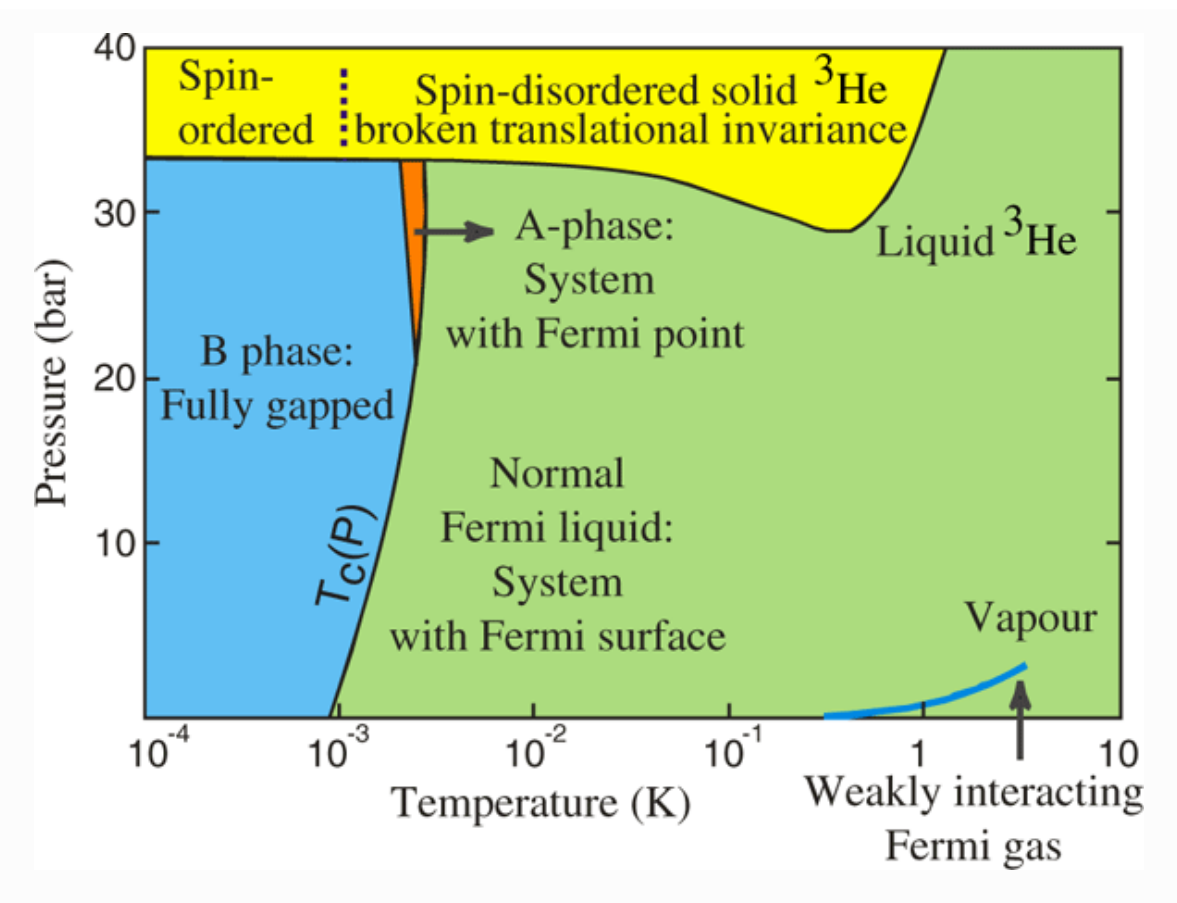
\includegraphics[width=0.62\textwidth]{figures/fig2_3.png}\\[2pt]
{\small 图 2.3：$^3$He 的相图（取自 [Vol09, 图 7.1]）}
\end{center}

\para{超流 $^3$He：}我们的最后一个例子是超流 $^3$He；它的理论可参看 [VW13, Vol09]。它的相图如图 2.3 所示。$^3$He 原子是自旋为 $1/2$ 的费米子，在低温下可以形成 Cooper 对。零磁场下有两个超流相，称为 A 相与 B 相。序参量（Cooper 对的期望值）取值于 $\C^3\otimes\C^3$，其中第一个因子对应自旋角动量，第二个因子对应轨道角动量，两者的自旋都为 1。把第一个 $\C^3$ 的基向量记为 $\mathbf{e}_{1,2,3}$，第二个的基向量记为 $\mathbf{f}_{1,2,3}$。自由能的对称群 $G$（忽略小的自旋--轨道耦合）由分别作用在 $\mathbf{e}_{1,2,3}$ 与 $\mathbf{f}_{1,2,3}$ 上的两个 $SO(3)$ 作用，以及一个公共的 $U(1)$ 相位旋转 $\mathbf{e}_i\otimes\mathbf{f}_j\mapsto c\,\mathbf{e}_i\otimes\mathbf{f}_j$ 给出。因此，自由能的对称性为
\begin{equation}
G=SO(3)\times SO(3)\times U(1). \tag{2.44}
\end{equation}

\begin{example}{2.40}
在 $^3$He 的超流相中，序参量取值
\begin{itemize}
\item A 相中为 $\mathbf{e}_1\otimes(\mathbf{f}_2+i\mathbf{f}_3)$；
\item B 相中为 $\sum_i\mathbf{e}_i\otimes\mathbf{f}_i$。
\end{itemize}
把这些序参量保持不变的子群记为 $H_{A,B}$，则势取极小的空间分别由 $G/H_A$、$G/H_B$ 给出。
\end{example}

% [原文 p.24]
\begin{question}{2.41}
尽可能显式地描述 $H_A$ 与 $H_B$。
\end{question}

你会看到，对称性破缺的模式与 QCD 中手征对称性的破缺非常相似。

有磁场时，还存在一个称为 $A_1$ 相的相。磁场把自由能的对称性降低到 $SO(2)\times SO(3)\times U(1)$，序参量取值
\[
(\mathbf{e}_2+i\mathbf{e}_3)\otimes(\mathbf{f}_2+i\mathbf{f}_3).
\]

继续之前，我们还有最后一个问题：

\begin{question}{2.42}
射影空间是齐性空间。你能把它们按齐性空间来描述吗？
\end{question}

\takeaway{本节用群作用的商构造流形：先给出作用、表示与商空间，再以射影空间和齐性空间为例。$\RP^n$、$\CP^n$、$\HP^n$ 是球面对 $O(1)$、$U(1)$、$Sp(1)$ 的商；对称性破缺的极小值空间是齐性空间 $G/H$。}

\section{不可定向曲面}

现在讨论一些不可定向流形。

\begin{example}{2.43}
考虑 $S^1\times[-1,1]$，用 $\theta\sim\theta+2\pi$ 与 $x\in[-1,1]$ 参数化。考虑 $\Z_2$ 作用 $(\theta,x)\mapsto(\theta+\pi,-x)$。商空间称为 Möbius 带。它不可定向，边界是单个圆 $S^1$。
\end{example}

作为不可定向闭流形，我们有上面引入的 $\RP^2$。为看出这一点，回想 $\RP^2=S^2/\Z_2$，其中 $\Z_2$ 作用把对径点等同。南半球上的任一点都与北半球上的某点等同。于是 $\RP^2$ 可以等同于北半球，而其边界（即赤道）带有额外的等同 $\theta\sim\theta+\pi$。

让我们更仔细地看赤道附近。可以用经度 $\theta$ 与纬度 $\phi\in(-\epsilon,\epsilon)$ 来参数化它。对径等同是 $(\theta,\phi)\sim(\theta+\pi,-\phi)$。这与 Möbius 带相同，而 Möbius 带不可定向。在弦论中，赤道附近的这种局部结构称为交叉帽（crosscap，原书夹注“叉帽”）。换一种说法：$\RP^2$ 是把北半球（即一个圆盘）沿边界粘到 Möbius 带上得到的。总结起来，

\begin{proposition}{2.44}
$\RP^2$ 不可定向。
\end{proposition}

另一种不可定向曲面可由如下商构造：

\begin{example}{2.45}
考虑用 $\theta$ 与 $\phi$ 参数化的 $T^2$，带有等同 $\theta\sim\theta+2\pi$、$\phi\sim\phi+2\pi$，并作如上的进一步等同：$(\theta,\phi)\sim(\theta+\pi,-\phi)$。结果称为 Klein 瓶。
\end{example}

在 $\phi=0$ 与 $\phi=\pi$ 附近，我们有两个 Möbius 带。所以所得曲面是把两个 Möbius 带沿边界粘起来。等价地，它是取连通和 $\RP^2\#\RP^2$ 得到的。

% [原文 p.25]
我们可以通过反复取连通和，考虑许多其他不可定向曲面：
\begin{equation}
\overbrace{\RP^2\#\RP^2\#\cdots\#\RP^2}^{h\ \text{个}}\#\overbrace{T^2\#T^2\#\cdots\#T^2}^{g\ \text{个}} \tag{2.45}
\end{equation}
其中 $h>0$、$g\ge0$。事实上，其中许多彼此同胚。

\begin{qmbox}\qmstmt{事实}{2.46}
任何紧连通不可定向二维曲面都同胚于
\begin{equation}
\RP^2\#\overbrace{T^2\#T^2\#\cdots\#T^2}^{g\ \text{个}} \tag{2.46}
\end{equation}
或 Klein 瓶 $\RP^2\#\RP^2$。
\end{qmbox}

证明 $\RP^2\#\RP^2\#\RP^2$ 同胚于 $\RP^2\#T^2$ 是有趣的练习。

\takeaway{本节讨论不可定向曲面：Möbius 带、$\RP^2$ 与 Klein 瓶。$\RP^2$ 由北半球与 Möbius 带沿边界粘成，赤道附近的局部结构称交叉帽。紧连通不可定向曲面都同胚于 $\RP^2\#T^2\#\cdots\#T^2$ 或 Klein 瓶。}

\section{附注：另一些有趣的流形}

\subsection{$\C^2/\Z_2$ 的消奇点}

考虑用 $(z,w)$ 参数化的 $\C^2$，以及 $\Z_2$ 作用 $(z,w)\mapsto(-z,-w)$。商空间 $\C^2/\Z_2$ 在原点奇异。我们可以用不同方式参数化同一空间：令 $(s,t,u):=(z^2,zw,w^2)$。于是 $\Z_2$ 作用在 $(s,t,u)$ 上是平凡的，但我们有关系 $su=t^2$。由满足 $su=t^2$ 的 $(s,t,u)$，可以唯一地重构 $(z,w)\simeq-(z,w)$。所以 $\C^2/\Z_2$ 可以等同于子空间
\begin{equation}
X=\{(s,t,u)\in\C^3\mid su=t^2\}. \tag{2.47}
\end{equation}
我们可以按如下方式消去 $X=\C^2/\Z_2$ 的奇点。

我们加入变量 $(x_1,x_2)\in\C^2\setminus\{0\}$，带等同 $(x_1,x_2)\sim a(x_1,x_2)$（$a\in\C\setminus\{0\}$）；也就是说，我们引入 $\CP^1\simeq S^2$。回想它的点记为 $[x_1:x_2]$。现在再加一个约束
\begin{equation}
(z,w)=c(x_1,x_2)\quad\text{对某个 } c\in\C, \tag{2.48}
\end{equation}
或等价地
\begin{equation}
(s,t,u)=c'(x_1^2,x_1x_2,x_2^2)\quad\text{对某个 } c'\in\C. \tag{2.49}
\end{equation}
把全空间记为 $\wt X$：它是 $\C^3\times\CP^1$ 的子空间，用 $(s,t,u,[x_1:x_2])$ 参数化，并受约束 $su=t^2$ 与式 (2.49)。这个空间带有两个投影映射：$\pi_1:\wt X\to X=\C^2/\Z_2$，由取 $(s,t,u)$ 给出；$\pi_2:\wt X\to\CP^1$，由取 $[x_1:x_2]$ 给出。% [Tutor Note: 原文此处误印作 \pi_2:X\to\CP^1，按上下文应为 \pi_2:\wt X\to\CP^1，译文从后者。]

注意 $\pi_1$ 除原点 $(z,w)=(0,0)$ 外是一一的。这是因为关系 (2.49) 唯一确定 $[x_1:x_2]=[z:w]$。在原点 $(z,w)=(0,0)$ 处，原像是整个 $\CP^1$。所以 $\wt X$ 可以看作在 $X=\C^2/\Z_2$ 的原点处插入了一个 $\CP^1$。

$\wt X$ 实际上是光滑流形。为看出这一点，考虑第二个投影 $\pi_2:\wt X\to\CP^1$。给定点 $[x_1:x_2]\in\CP^1$，$\pi_2$ 的原像就是 $c'(x_1^2,x_1x_2,x_2^2)\in\C$（$c'\in\C$）。所以它同构于一份 $\C$。于是 $\wt X$ 可以看作在 $\CP^1$ 的每一点处光滑地粘上一份 $\C$，从而是光滑流形。这是我们下一节要讨论的纤维丛的一个例子。

% [原文 p.26]
\subsection{一个 K3 流形}

上面引入的流形 $\wt X$ 非紧。它可以用来构造一个相当重要的四维紧流形。从 $T^4$ 出发，用 $\theta_i\in\R$ 参数化，带等同 $\theta_i\sim\theta_i+2\pi$，$i=1,2,3,4$。考虑由
\begin{equation}
(\theta_1,\theta_2,\theta_3,\theta_4)\mapsto-(\theta_1,\theta_2,\theta_3,\theta_4) \tag{2.50}
\end{equation}
给出的 $\Z_2$ 作用。

注意在等同 $\theta\sim\theta+2\pi$ 下，$\theta\sim-\theta$ 当且仅当 $\theta=0,\pi$。因此当 $\theta_i=0,\pi$（$i=1,2,3,4$）时，商空间 $T^4/\Z_2$ 在 $2^4=16$ 个点处奇异。在每个点附近，它局部具有上面研究过的形式 $\R^4/\Z_2=\C^2/\Z_2$。于是可以在这 16 个点处各插入一份 $\CP^1$ 来消奇点。结果是四维光滑紧流形，属于一类称为 K3 的流形。\footnote{K3 这个名字是数学家 A. Weil 起的：它来自研究过它的三位数学家 Kummer、Kähler 与 Kodaira，也来自喜马拉雅山的 K2 峰。这里给出的构造归功于 Kummer。}

\takeaway{本节给出两个附注例子：$\C^2/\Z_2$ 在原点插入一个 $\CP^1$ 后消去奇点，得到纤维丛；$T^4/\Z_2$ 的 16 个奇点各插入一个 $\CP^1$，得到四维紧流形 K3。}

\section{附注：关于流形的一些奇特事实}

\subsection{光滑流形与拓扑流形}

考虑 $\C^5$ 中的方程
\begin{equation}
z_1^2+z_2^2+z_3^2+z_4^3+z_5^{6k-1}=0. \tag{2.51}
\end{equation}
除原点外，它是复四维（即实八维）的光滑流形。我们可以取它与 $\C^5$ 中单位球面 $S^9=\{\sum|z_i|^2=1\}$ 的交。这给出一个七维光滑紧流形 $M_k$。已知所有 $M_k$ 都同胚于标准 $S^7$，但除非 $k$ 是 28 的倍数，它们与 $S^7$ 不微分同胚。事实上，把 $S^7$ 做成光滑流形恰好有 28 种方式，而上述构造把它们穷尽了。这要追溯到 Milnor 1956 年的工作；一个很好读的叙述可参看 [Mee17]。这些流形称为异种球面，但它们并不很奇怪，上面的显式方程就说明了这一点！

也存在拓扑流形不容许任何光滑结构的情形。这样的四维流形是 Freedman 在 1982 年发现的 [Fre82]。一个例子称为 $E_8$ 流形。同样，用坐标卡以及它们之间连续映射的构造是显式的；困难之处在于证明不可能存在任何光滑结构。次年，即 1983 年，Donaldson [Don83] 引入了用规范理论研究光滑四维流形的新方法，得到许多引人注目的结果。很快发现的一个结果是：$\R^4$ 也存在与标准结构不微分同胚的光滑结构。（例如，在其中一种异种光滑结构中，任何光滑嵌入的 $S^3$ 都位于原点附近的一个紧区域内。因此其中不可能有任意大的 $S^3$。）

\subsection{流形的三角剖分}

二维曲面可以三角剖分。在更高维可以问同样的问题，只是把三角形换成单形。（$n$ 维单形有 $n+1$ 个顶点，等等。）流形可以三角剖分吗？已知光滑流形可以三角剖分。拓扑流形呢？

% [原文 p.27]
嗯，上面的四维 $E_8$ 流形不能三角剖分。五维以上情形更微妙。Matumoto 在 1978 年 [Mat78] 与 Galewski--Stern 在 1980 年 [GS80] 证明：如果存在一个满足某些性质的三维流形，那么所有 $n\ge5$ 维拓扑流形都可以三角剖分。若不存在这样的三维流形，则对每个 $n\ge5$，都有不能三角剖分的拓扑流形。这种三维流形的不存在性，最终由 Manolescu 在 2013 年证明 [Man13]。这项工作用到了 Seiberg--Witten 理论的数学版本，而该理论起源于理论物理中 Seiberg 与 Witten 于 1990 年代中期对超对称规范理论的研究；他们说明了禁闭如何在 QCD 的超对称版本中发生。这套数学上的 Seiberg--Witten 理论可以看作上面提到的 Donaldson 理论的简化版本，自提出以来已被数学家大力研究。

\subsection{一些评论}

于是流形上的结构有一个层级：
\begin{equation}
\begin{aligned}
&\{\text{拓扑流形}\}\supset\{\text{三角剖分流形}\}\\
&\qquad\supset\{\text{PL 流形}\}\supset\{\text{光滑流形}\}
\end{aligned}\tag{2.52}
\end{equation}
其中我加上了另一层，即分段线性（PL）流形；它在数学文献中比三角剖分流形更常见。\footnote{PL 流形是满足下述条件的三角剖分流形：对每个顶点 $v$，$v$ 的链环（由紧邻 $v$ 的单形构成的多面体）分段线性同构于 $S^{n-1}$。}如上所见，每一层都有各种差别。

我为什么关心这些？我并不真的知道。但让我给一些理由。

\begin{itemize}
\item 首先，它本身就有趣，至少对我而言。
\item 其次，特别有趣的是，研究这些问题用到了规范理论（因而受物理启发）的方法。
\item 第三，我注意到高能物理（hep-th）与凝聚态物理（cond-mat）的人之间有如下差别：在高能物理中，我们常把光滑流形当作给定的（如同广义相对论中）；而在凝聚态物理中，流形只作为更基本的晶格结构的远程近似出现。在理论凝聚态物理中，研究一般流形时常常假定它带有三角剖分。因此我认为，了解处理流形的这两种方式之间的区别或许有用。例如，似乎可以为某种奇异的对称保护拓扑相写下哈密顿量，它定义在三角剖分流形上，从而能探测非光滑但可三角剖分的流形，所用的是一个称为 Kirby--Siebenmann 类的示性类。不过，这给出的是在我们的实际世界中毫无意义的相当高维的模型。
\end{itemize}

\takeaway{本节列举奇特事实：七维球面恰有 28 种光滑结构；四维存在不容许光滑结构的拓扑流形（$E_8$ 流形）；五维以上的三角剖分问题由 Manolescu 解决。章末给出拓扑、三角剖分、PL、光滑四层结构的层级。}

\chapterreview{本章引入流形：每点局部同胚（或微分同胚）于 $\R^n$ 的开集，坐标卡之间由转移函数粘接，紧流形可由有限个坐标卡覆盖。流形有三种常见造法：方程的零点集，乘积、连通和等组合操作，以及群作用的商。由此得到球面、环面、群流形 $O(n)$、$U(n)$、$Sp(n)$，以及射影空间和齐性空间；后者正描述了对称性破缺后势的极小值空间。章末讨论不可定向曲面，并以附注形式介绍消奇点、K3 流形、异种球面与三角剖分问题。光滑流形与拓扑流形的差别贯穿全章，后面讨论拓扑相时会再遇到。}
